\chapter{系统设计与实现}
\section{开发环境}
\subsection{硬件环境}
这个实验是靠性能比较强的本地计算机来完成的,它主要的硬件配置情况如下所示,处理器选用的是Intel Core i9这款产品,它具备多核心以及高主频的特性,能够支持复杂计算任务和高并发程序运行,显卡采用的是NVIDIA GeForce RTX 3060这一型号,具备较强的图形渲染与并行计算方面能力,有利于运行自动驾驶模拟平台比如CARLA 0.9.13和进行深度学习模型推理,内存大小达到了32GB这样的容量,大容量内存保证了在多线程和大数据处理时系统流畅性,能有效避免出现内存瓶颈方面的相关问题,这样的硬件配置为自然语言场景生成、自动驾驶仿真以及模型评估等任务提供稳定且高效运行环境。
\subsection{软件环境}
系统开发和运行所基于的操作系统是 Windows 11,其为微软最新发布出来的操作系统,能提供良好的用户体验以及强大的系统性能,并且和各类开发工具与依赖库具备广泛兼容性,它支持多种编程语言以及开发框架,可满足项目开发过程里的各种需求。

项目主要是将 Python 3.8 作为开发语言来运用,Python 属于一种被广泛使用的高级编程语言,它凭借简洁的语法以及强大的库支持而闻名于世,在自然语言处理、机器学习和自动驾驶仿真等诸多领域均有广泛应用,Python 3.8 能够提供稳定的语言特性和相关优化,可满足项目开发过程中的各类实际需求。

软件环境需要的依赖库方面已经安装好,具体如下表所示:
\begin{table}[H]
	\centering
	\begin{tabular}{lll}
		\hline
		\small % 设置表格字体大小为小号
		\textbf{库名称} & \textbf{版本} \\
		\hline
		openai & 最新版本 \\
		sentence\_transformers & 最新版本 \\
		torch & 1.13.1+cu117 \\
		torchvision & 0.14.1+cu117 \\
		torchaudio & 0.13.1 \\
		gym & 0.23.1 \\
		numpy & 1.21.6 \\
		pygame & 2.3.0 \\
		tqdm & 4.65.0 \\
		pyyaml & 6.0 \\
		matplotlib & 3.5.3 \\
		opencv-python & 4.7.0.72 \\
		pandas & 1.5.3 \\
		seaborn & 0.12.2 \\
		shapely & 1.8.5 \\
		ephem & 4.1.4 \\
		joblib & 1.2.0 \\
		cpprb & 10.7.0 \\
		pycocotools & 2.0.6 \\
		moviepy & 1.0.3 \\
		scikit-image & 0.19.3 \\
		transformers & 最新版本 \\
		setGPU & 最新版本 \\
		\hline
	\end{tabular}
	\caption{项目依赖库及其版本}
	\label{tab:dependencies}
\end{table}


\section{系统核心功能实现}
\subsection{自然语言理解功能}
在自然语言输入这方面首先要了解到的就是测试数据,其是为了综合体现自动驾驶场景多样复杂特点,涵盖像直行障碍、转弯障碍等多种典型场景类别,例如直行障碍、转弯障碍、变道、超车、闯红灯、无保护左转、右转以及交叉路口协商等,这些场景类别覆盖自动驾驶车辆实际道路环境可能遇到的关键交互情况,具备较高代表性和实用价值。数据集中场景描述以自然语言形式进行呈现,并且包含一定比例模糊性描述,以此模拟真实世界里驾驶员或其他交通参与者行为不可预测性,场景描述模糊性设计有助于测试生成系统应对不精确指令时的处理能力,确保系统能够适应并生成符合要求的复杂交通场景。
\begin{figure}[H]
	\centering
	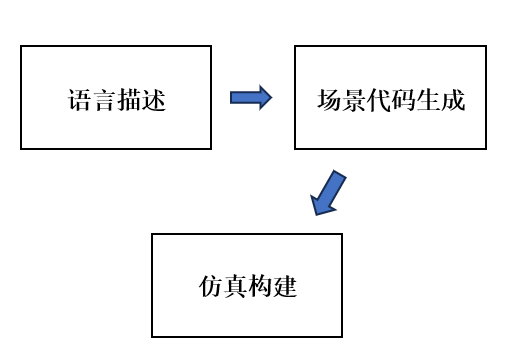
\includegraphics[width=0.7\textwidth]{"images/流程图1.pdf"}
	\caption{从自然语言描述到仿真场景构建的流程图}
	\label{fig:flowchart}
\end{figure}

本模块负责接收自然语言输入并生成对应的Scenic场景描述。具体流程如下:

输入:自然语言形式的场景描述,例如“The ego vehicle is driving on a straight road; the adversarial pedestrian suddenly appears from behind a parked car on the right front and suddenly stop.”。
检索增强:使用 \texttt{sentence-transformers} 中的 \texttt{sentence-t5-large} 模型对输入进行向量化表示,并在本地检索数据库(如 \texttt{retrieve/scenario\_descrip\\tions.txt})中查找相似描述作为参考样本。
大语言模型解析:采用预训练的大语言模型(如 GPT-4o),结合检索到的参考样本,生成符合输入语义的 Scenic 脚本。
场景拼接机制:根据场景复杂度,支持对多个子元素(如车辆、行人、环境条件)进行组织与拼接。



\subsection{场景合成与仿真模块}

本模块承担着把自然语言生成的Scenic脚本转化成三维可视化仿真场景的任务,并且要在CARLA仿真平台上达成动态运行,整个流程涵盖脚本解析、场景构建、仿真控制、交互支持以及数据输出等多个环节,具体情况如下:

Scenic解析:本系统会先借助Scenic内置的语法与语义分析器来对输入脚本开展解析工作,Scenic作为一种领域专用语言可让用户用简洁且结构化的方式去描述场景元素像车辆、行人、障碍物等的初始状态和约束条件,解析过程能够生成涵盖对象属性如位置、速度、朝向以及交互规则如跟车距离、避让行为还有环境条件如天气、时间的完整场景配置

仿真构建:完成脚本解析之后系统自动把Scenic生成中间配置映射到CARLA仿真平台里,具体涵盖载入指定地图、部署交通参与者、设定摄像头和LiDAR等传感器参数、配置天气光照路况等环境因素等内容,系统能够依据配置实现对城市道路高速公路十字路口等多种类型场景精准建模
接口调用关系:Scenic借助和CARLA集成的Python API来调用底层仿真接口,系统会自动完成Actor的创建以及状态初始化和行为脚本绑定等任务,这极大程度简化了从脚本到仿真的转换流程,研究人员不用手动编程就能通过文本控制仿真流程,显著提升了效率和复用性。

动态交互支持:系统能够支持高度动态化的场景仿真工作,还可以模拟交通参与者之间的交互行为,像车辆变道、避障、红绿灯响应以及行人横穿马路等情况,Scenic语言提供了条件触发与时间控制相关机制,允许用户描述复杂的行为序列内容,以此实现具有时序性、可演化的场景变化状况,从而增强了仿真的真实感与复杂程度。

多样化仿真配置模块能灵活进行仿真参数配置,涵盖地图选择像Town01、Town05等类型,包含天气设置有晴天、雨天、雾天等情况,还有交通流量控制以及车辆控制模式如自动驾驶、手动控制等内容,可满足不同测试需求,且该模块支持不同版本CARLA和Scenic组合使用,具备较好兼容性与可拓展性。


输入数据:本实验采用约20条自然语言描述作为输入样本,用于生成自动驾驶场景。这些描述覆盖多种交通情境和突发事件,例如:

(1)自车在红绿灯前等待信号

(2)行人突然横穿街道

(3)The ego vehicle is driving on a straight road; the adversarial pedestrian appears from a driveway on the left and suddenly stop and walk diagonally.

(4)The ego vehicle is driving on a straight road when a pedestrian suddenly crosses from the right front and suddenly stops as the ego vehicle approaches.

下面我用一个具体的例子展示我是如何实现carla场景生成的,
\textbf{场景描述:} 自车在直路上行驶时,一名行人突然从右前方穿出

\indent (自然语言输入)The ego vehicle is driving on a straight road when a pedestrian suddenly crosses from the right front and suddenly stops as the ego vehicle approaches.\\
\begin{lstlisting}[language=Python, caption={场景关键代码示例}, label={lst:scenic_key}, numbers=left, xleftmargin=2em]
	behavior AdvBehavior():
	do CrossingBehavior(ego, globalParameters.OPT_ADV_SPEED, globalParameters.OPT_ADV_DISTANCE) 
	until (distance from self to egoTrajectory) < globalParameters.OPT_STOP_DISTANCE
	while True:
	take SetWalkingSpeedAction(0)
	
	ego = Car at EgoSpawnPt,
	with heading yaw,
	with regionContainedIn None,
	with blueprint EGO_MODEL
	
	IntSpawnPt = OrientedPoint following roadDirection from EgoSpawnPt 
	for globalParameters.OPT_GEO_Y_DISTANCE
	AdvAgent = Pedestrian right of IntSpawnPt by globalParameters.OPT_GEO_X_DISTANCE,
	with heading IntSpawnPt.heading + 90 deg,
	with regionContainedIn None,
	with behavior AdvBehavior()
	
	require (distance from AdvAgent to intersection) > 10
\end{lstlisting}
\begin{figure}[H]
	\centering
	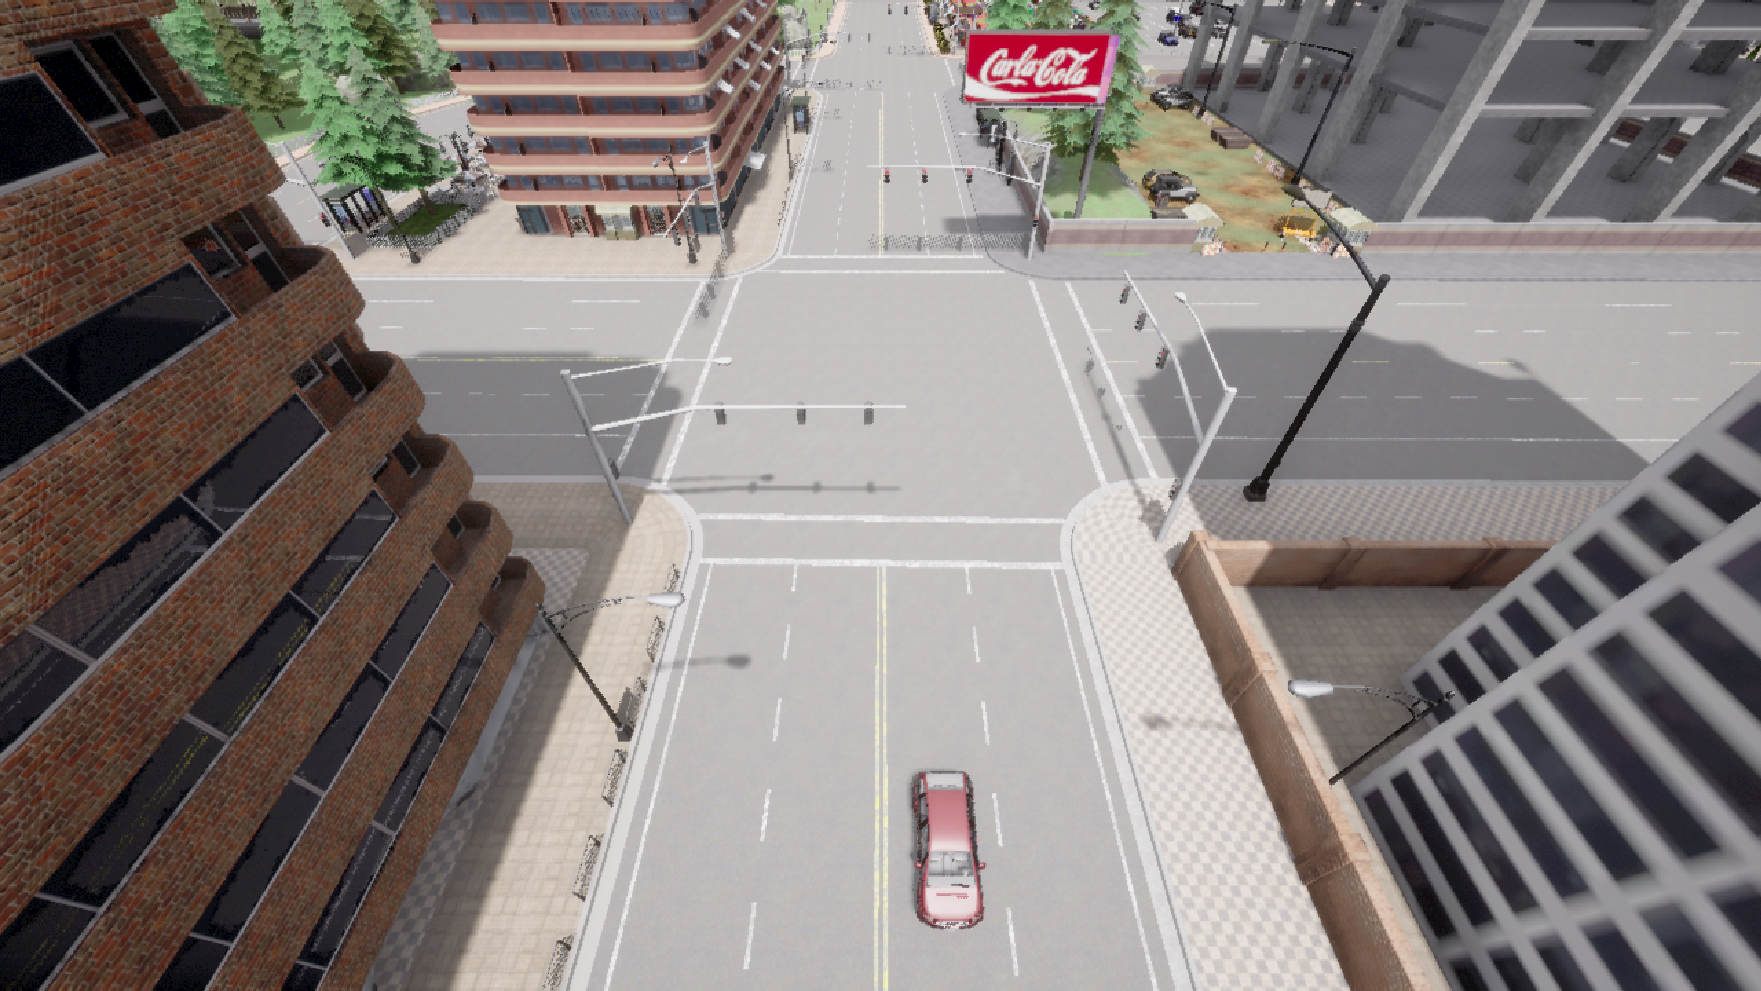
\includegraphics[width=0.8\textwidth]{"images/场景5.pdf"}
	\caption{场景截图}
	\label{}
\end{figure}
调用生成的scenic代码,实现仿真模拟脚本,以及场景保存。
\subsection{场景评估与展示模块}

场景评估与展示模块的目的是对生成的三维仿真场景做可视化呈现和定量分析,此模块方便研究人员直观了解场景生成具体效果,也为后续性能比较、模型调优以及系统验证提供评估依据,该模块包含下面几个关键功能:


可视化展示:在仿真进行的过程当中系统能够自动截取关键帧的截图,或者录制完整的仿真过程视频并保存成图像或视频文件,截图一般会选择交通事件发生点像刹车、避障、碰撞等情况,或者特定的时序节点,以此确保所展示信息具备代表性与丰富性,视频部分可以借助CARLA原生录制功能或者集成第三方渲染引擎来实现,并且支持多角度、多摄像机的可视观察,从而进一步增强场景调试与验证方面的可操作性。

评价指标主要涵盖安全性、驾驶性能、场景语义一致性和系统鲁棒性等多个方面,安全性指标包含碰撞次数、闯红灯次数、交通规则违章等内容,用来衡量系统的安全保障能力,驾驶性能指标诸如轨迹偏差、车道保持率和速度控制平稳性,反映车辆行驶的准确性和舒适度,场景语义一致性指标评估生成场景与自然语言描述的匹配度及多样性,系统鲁棒性指标关注系统在异常情况下的恢复能力及对复杂环境的适应性,综合这些指标能够全面量化自动驾驶系统在不同测试场景中的表现并指导系统优化与改进。

量化评估:本系统是在自动化生成以及仿真的基础之上,进一步引入多维度的量化评估指标,以此对场景生成的有效性、合理性和多样性进行定量测量,具体涵盖的内容有:

(1)语义保真度(Semantic Fidelity):这个指标的作用是衡量输入的自然语言描述和最终生成的仿真场景之间语义一致性,可采用人工标注评分和自动化匹配算法相结合的方式来开展,比如通过设定关键语义要素像地点、交通行为、天气条件等的匹配程度,对场景是否准确还原用户意图进行评分,自动方法能够结合自然语言处理与图结构匹配技术实现初步评估进而提升效率。


(2)多样性指标(Scene Diversity):这项指标能反映系统生成场景在多次输入不同自然语言之后的差异性以及覆盖范围,主要涵盖空间多样性像不同地图位置与道路类型等方面、元素多样性比如参与车辆行人非机动车种类情况、行为多样性包含速度控制路线选择交通交互等内容,统计方法有使用Shannon熵、Jaccard相似度或者聚类分布指标等,以此全面反映生成系统的泛化能力和表现范围。

(3)驾驶性能指标(Driving Performance):为了评估生成场景对自动驾驶系统测试价值,本模块支持在生成场景里运行预设自动驾驶控制系统,像基于CARLA的自动驾驶Agent并记录其表现,关键评估维度包含碰撞率也就是单位场景中发生碰撞的比例、任务成功率即是否成功完成任务或驶出场景、路径偏离率指与理想路径的偏差程度等,这些数据能够用于评估生成场景的挑战性与安全测试覆盖度,是场景质量评估的重要依据。

评估结果展示与导出:系统将展示代码运行出的评估结果用列出的形式来做可视化展示,所有截图、评估指标还有分析数据都可以导出成标准格式文件,例如CSV、JSON、PNG等,可用于论文撰写、模型调试或者进一步的数据挖掘。

\begin{table}[H]
	\centering
	\caption{系统评估结果}
	\label{tab:evaluation_results}
	\begin{tabular}{lc}
		\toprule
		指标名称 & 数值 \\
		\midrule
		碰撞率 (collision\_rate) & 0.0 \\
		红灯违规频率 (avg\_red\_light\_freq) & 0.0 \\
		停车标志违规频率 (avg\_stop\_sign\_freq) & 0.0 \\
		出路面长度 (out\_of\_road\_length) & 0.0 \\
		路线跟踪稳定性 (route\_following\_stability) & 0.806 \\
		路线完成度 (route\_completion) & 0.93 \\
		平均时间消耗 (avg\_time\_spent) & 4.5 \\
		平均加速度 (avg\_acceleration) & 0.32 \\
		平均偏航角速度 (avg\_yaw\_velocity) & 0.0 \\
		车道入侵频率 (avg\_lane\_invasion\_freq) & 0.0 \\
		安全操作得分 (safety\_os) & 1.0 \\
		任务完成得分 (task\_os) & 0.802 \\
		舒适度得分 (comfort\_os) & 1.0 \\
		最终综合得分 (final\_score) & 0.941 \\
		\bottomrule
	\end{tabular}
\end{table}

在这个示例评估里系统展现出较高安全性,碰撞率和交通违规频率两个数据均为零,这表明系统在基础安全保障方面表现相当不错,路线跟踪稳定性达到大约0.81这个数值,显示系统具备较好的路径跟踪能力,路线完成度或许意味着按预定路线行驶情况良好,安全操作和舒适度的得分都拿到了满分,说明车辆运行状态平稳且符合安全标准,最终综合得分是0.94这个成绩,整体表现算得上优秀但仍有提升空间,尤其是在任务完成度这一方面。




\section{系统编码与实现}

\subsection{系统整体架构与主程序设计}

本系统基于 Python 语言开发,结合 Carla 0.9.13 与 SafeBench 框架,整体架构模块化且层次清晰。系统以两个主控脚本 \texttt{run\_train.py} 和 \texttt{run\_train\_dynamic.py} 作为入口,分别负责仿真评估与动态场景训练。参数统一通过 \texttt{argparse} 管理,涵盖实验配置、设备选取、模型路径、输出目录等,保障了实验的灵活性和复现性。

在整体的运行流程当中,系统会先依据传入的配置文件去加载代理(Agent)和场景参数,之后按照策略类型自动选择对应的运行器(Runner)并启动仿真过程,同时在设计里充分考虑了配置文件路径的动态拼接以及输出目录的自动创建,以此确保文件管理的规范与安全。

\begin{verbatim}
	# 伪代码:主程序执行流程
	parse_args()
	for each agent_cfg in agent_cfg_list:
	for each scenario_cfg in scenario_cfg_list:
	set_device_and_seed()
	agent_config = load_config(agent_cfg)
	scenario_config = load_config(scenario_cfg)
	setup_output_dirs()
	if scenario_config.policy_type == 'scenic':
	runner = ScenicRunner(agent_config, scenario_config)
	else:
	runner = CarlaRunner(agent_config, scenario_config)
	runner.run()
\end{verbatim}

\subsection{主控脚本功能与运行流程}

\texttt{run\_train.py} 支持三种主要模式:代理训练(\texttt{train\_agent})、场景训练(\texttt{train\_scenario})和评估(\texttt{eval}),并依据配置自动调用 \texttt{CarlaRunner} 或基于 Scenic 场景语言的 \texttt{ScenicRunner}。该设计方便用户针对不同实验需求进行灵活切换。

而 \texttt{run\_train\_dynamic.py}则专注于依据自然语言描述开展动态场景训练,默认加载动态场景的配置文件,实现自然语言到Scenic代码的实时转换,自动创建和训练相关的模型保存路径,以此确保训练过程的中断恢复与结果管理。
两者均利用多线程控制计算资源,支持 GPU 设备切换,并可选渲染和视频保存,为仿真结果的展示和后期分析提供便利。

\subsection{动态场景仿真控制与异常处理}

动态场景仿真是系统的关键模块,基于 \texttt{ScenicRunner} 的扩展实现。系统会接收自然语言所做的描述,然后经过预处理与解析的步骤,将其转换成 Scenic 语言脚本内容,接着由运行器对脚本进行加载并执行,最终自动生成符合语义要求的三维交通场景。

在仿真流程里系统会对每个场景实例做初始化,载入车辆、传感器以及任务配置等内容,并且严格把控仿真时长和步长,为保障系统具备健壮性引入了异常捕获机制,可捕获并打印详细异常堆栈信息,还能保证后续实验连续执行 。

\begin{verbatim}
	# 伪代码:动态场景仿真异常处理
	try:
	runner.run(test_epoch)
	except Exception as e:
	runner.close()
	log_error(traceback.format_exc())
	continue_with_next_experiment()
\end{verbatim}

本系统借助合理设计出来的主程序结构、配置管理以及动态场景运行机制,达成了从自然语言描述到三维智能驾驶仿真的高效转换,为智能驾驶仿真研究和场景生成提供强有力的技术支撑。
